% !TEX root = ../thesis.tex

%%%%%%%%%%%%%%%%%%%%%%%%%%%%%%%%%%%%%%%%%%%%%%%%%%%%%%%%%%%%%%%
% Chapter: Performance Overhead
%%%%%%%%%%%%%%%%%%%%%%%%%%%%%%%%%%%%%%%%%%%%%%%%%%%%%%%%%%%%%%%

\chapter{Performance Overhead}\label{appdx:PerformanceOverhead}

After a simple experiment we collected data in order to show the overhead introduced by using reflection and dynamic proxies in managed data.
The experiment is performed on the application of the example explained in Chapter \ref{Example Application}, its simple version.
We have implemented a second version of this state machine application in pure Java, the main code however remained exactly the same.

In order to collect data for performance over head we ran the two applications using simple profiler code, which just measures the start and the end time of the application and presents the difference.
We have measured four different versions of the application.
First, the pure Java application, in order to show what is the ``real'' execution duration.
Second, the Managed Data version complete.
Third, the Managed Data version excluding the bootstrapping process, which is very slow.
Finally, the Managed Data version excluding the bootstrapping and the schema loading process, which is performed once and also introduces a significant performance overhead.
This last version should be the closest to the original one since all the ``heavy'' processes have been excluded.
The experiment consisted of a 10 times execution of each application versions.
Figure \ref{fig:Performance Overhead} illustrates the performance overhead that managed data introduce by showing the average execution time duration.

\begin{figure}[H]
	\centering
	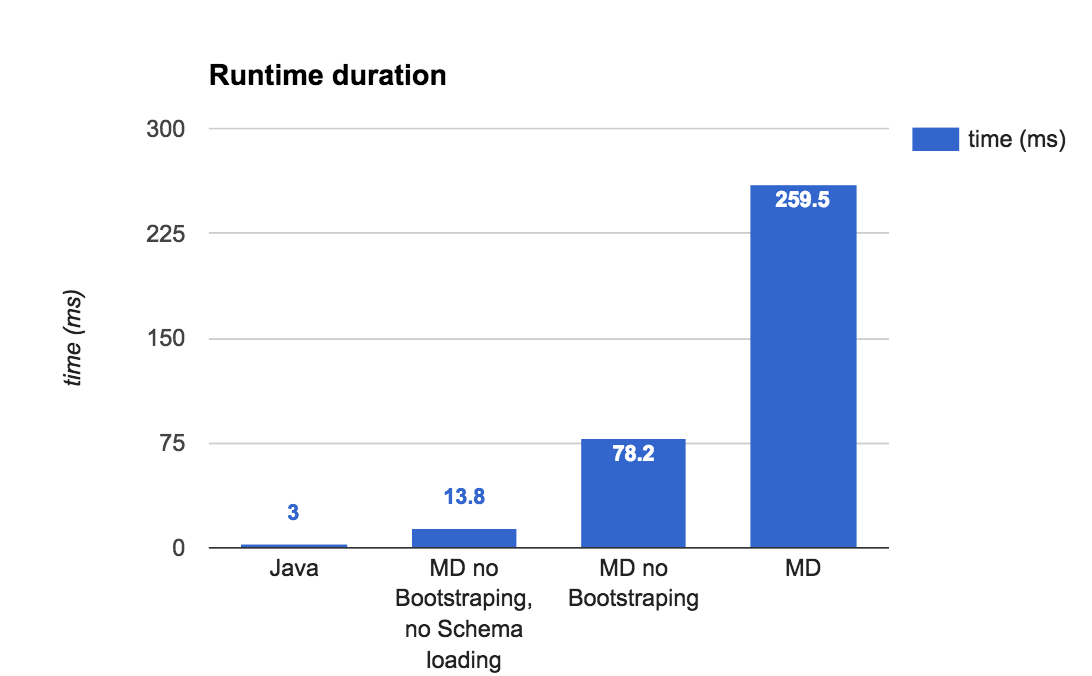
\includegraphics[scale=0.5]{figures/PerformanceOverhead.png}
	\caption{Performance Overhead}
  	\label{fig:Performance Overhead}
\end{figure}

As the figure shows the managed data version even without the bootstrapping and schema loading processes, has 4-5 times larger execution time.
Next, in the case where the bootstrapping is excluded, which in real cases it is going to performed only once in the beginning, the execution time is 6 times larger from the managed version that includes bootstrapping and almost 26 times larger than the pure Java version.
Finally, if both bootstrapping and schema loader is included in the measurement, the numbers are impressively large. 
However, optimizations like loading every managed data upfront during the beginning of the application would help, the time in this case would fall to the second case, which is still a significant overhead but more acceptable.